\chapter{Results}\label{results}
This chapter discusses the results we obtained by processing data using the HCP pipelines. The differences we observed and the quantified metric values are discussed in detail for each pipeline. Section \ref{sec:Prefreesurfer} discusses PrefreeSurfer results, followed by section \ref{sec:Freesurfer} on FreeSurfer results, section \ref{sec:Postfreesurfer} on PostFreeSurfer results, section \ref{sec:fMRI} discusses fMRIVolume pipeline results and section \ref{sec:comparison} compares the effect of operating systems on HCP pipelines against the anatomical variations in the subjects.

\section{PreFreeSurfer} \label{sec:Prefreesurfer}
The subjects were processed on CentOS6 and CentOS7 using the PreFreeSurfer pipeline. Among the 92 NIfTI imaging files common to all 5 subjects, 76 (.nii.gz) files differed between CentOS6 and CentOS7. Figure~\ref{fig:prefreesurfer_metric_values} shows the Dice coefficient and NRMSE values of the NIfTI files that were found to have differences in between operating systems.

\subsection{Global comparison}
The general findings about the differences in the output images due to the PreFreeSurfer processing is discussed in this section.

\begin{center}
\begin{tabular}{|l|l|l|}
\hline
\textbf{Item}      & \textbf{Nrmse} & \textbf{Dice} \\ \hline
Mean               & 0.0088   & 0.3212   \\ \hline
Median             & 0.0043    & 0.0557    \\ \hline
Standard Deviation & 0.0160    & 0.3806   \\ \hline
\end{tabular}
\captionof{table}[NRMSE \& DICE values of PreFreeSurfer]{NRMSE \& DICE values of PreFreeSurfer processing on CentOS6 and CentOS7}
\label{tab:PreFreeSurfer_Metic_Values}
\end{center}

Table \ref{tab:PreFreeSurfer_Metic_Values} contains the average mean, median and standard deviation we calculated for the metrics, NRMSE value and Dice coefficient. Dice coefficient shows that out of the results we obtained from PreFreeSurfer processing on two conditions, there was only 32\% similarity while taking the average of Dice coefficient of every file that we found to have a checksum difference.

\begin{center}
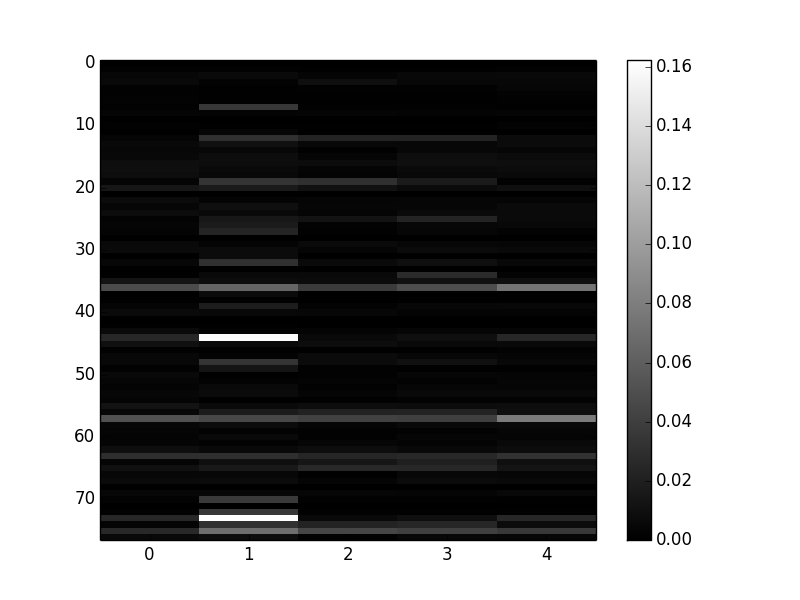
\includegraphics[width=.5\linewidth]{prefreesurfer_nrmse.png}%
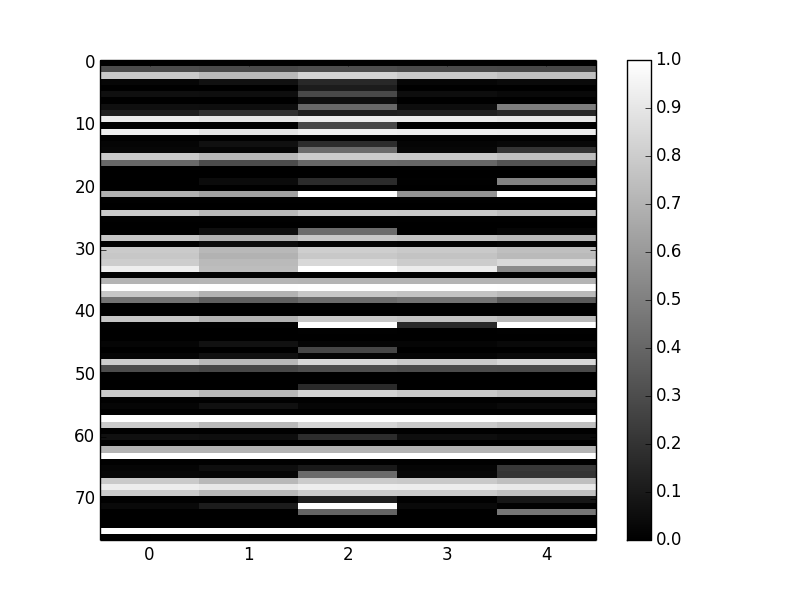
\includegraphics[width=.5\linewidth]{prefreesurfer_dice.png}
\captionof{figure}[PreFreeSurfer metric values]{PreFreeSurfer metric values\\(i) NRMSE (left) (ii)Dice coefficient (right)}
\label{fig:prefreesurfer_metric_values}
\end{center}

Figure \ref{fig:prefreesurfer_metric_values} contains the matrices showing the plotted values of NRMSE (left) and Dice Coefficient (right).
Each line in the matrix corresponds to a file common to all the subjects.
Each column represents a subject and each row represents the same file in 5 different subjects. The files are sorted according to their modification time.
The NRMSE value appears brighter if the images are dissimilar and it appears darker if the images are similar. Conversely, the Dice coefficient value appears darker if the images are dissimilar and appears brighter if the images are similar. We can also observe that the magnitude of differences varies across the files as well as the subjects.

\subsection{Comparison of specific files}
Figure~\ref{fig:prefreesurfer_t1w_mul} illustrates the differences in the ``T1wmulT2w\_brain\_norm\_s5.nii.gz" file. This file gets created as part of bias field correction (step (10), Figure \ref{fig:prefreesurfer_overview}). Figure~\ref{fig:prefreesurfer_t1w_mul} is a checkerboard image with a patch size 5. Checker board image is created by alternating between the patches belonging to two different images. No two adajacent squares would belong to the same image.
The file was taken from BiasFieldCorrection\_sqrtT1wXT1w folder in subject ``101410". File has an NRMSE value of 0.009 and the Dice coefficient value is 0.328. Small squares in the figure indicates the differences. Figure~\ref{fig:prefreesurfer_zoom} shows the zoomed version of part of the checkerboard image marked by red square in Figure~\ref{fig:prefreesurfer_t1w_mul}.
The link given below at the caption of the image contains the CentOS6 and CentOS7 files alternating in between each other. We can identify the differences around the border visually.

\begin{center}
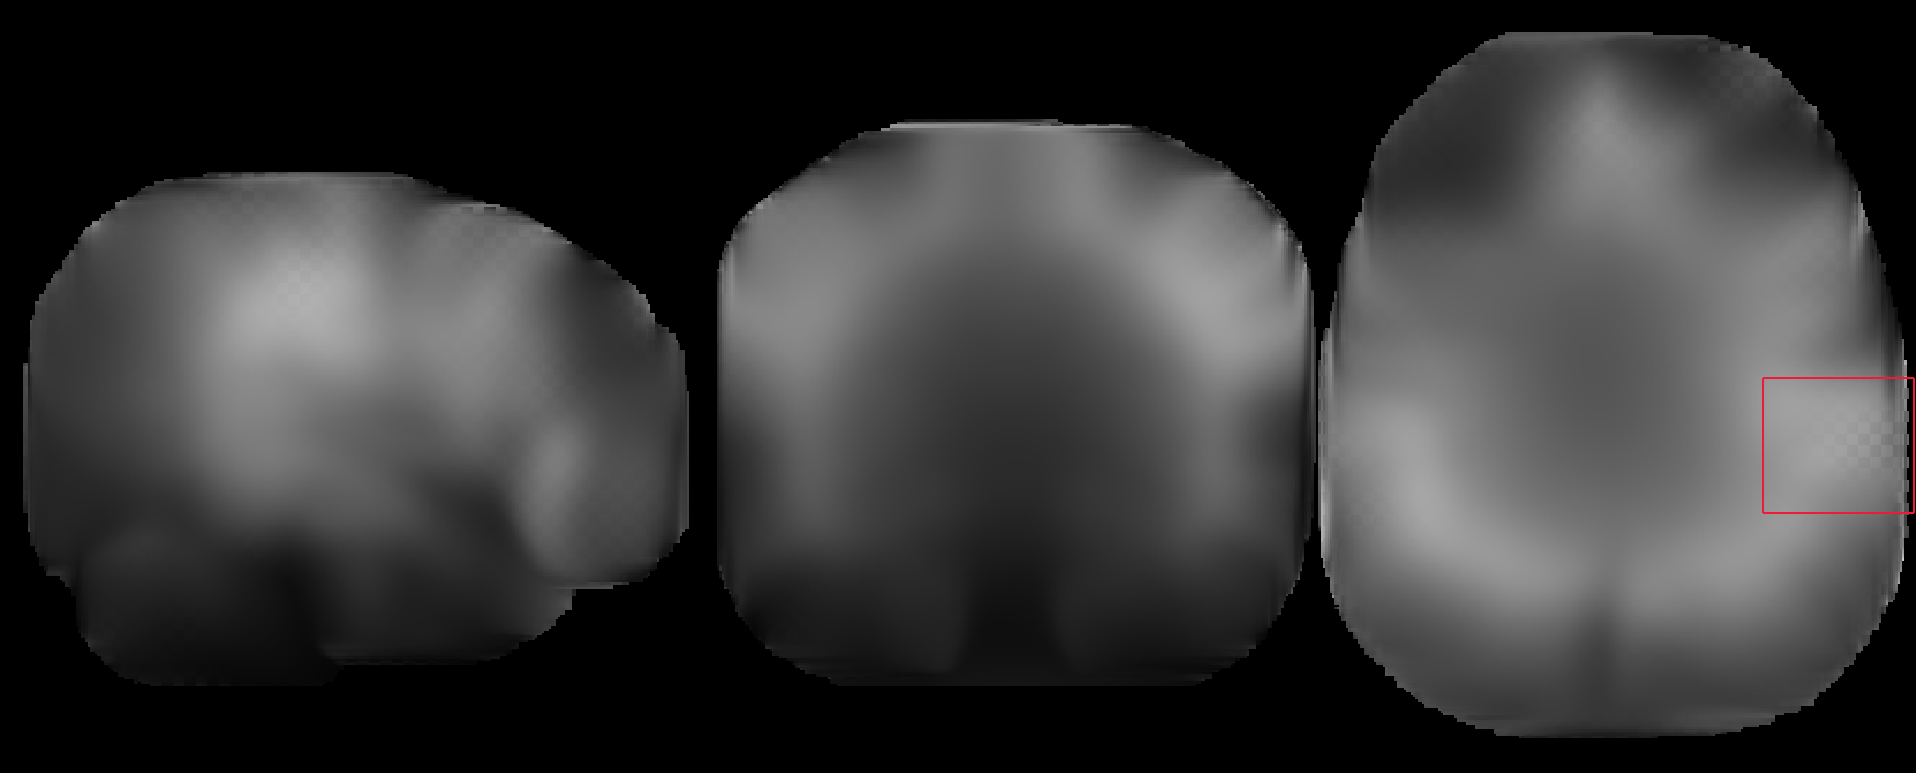
\includegraphics[width=.9\linewidth]{t1wmul_checkerboard_patchsize5_copy.png}
\captionof{figure}[Differences in T1wmulT2w brain normalization file]{Differences in T1wmulT2w brain normalization file (checkerboard image). \href{https://drive.google.com/file/d/1eHyrs180QbF4a-kSSz5mFkdirTgdXhc_/view?usp=sharing}{Link to the animated illustration of differences}.\\Figure~\ref{fig:prefreesurfer_zoom} shows the zoomed version of part of the image marked by the red square.\\(Subject: 101410; Filename: T1wmulT2w\_brain\_norm\_s5.nii.gz; Dice coeff.: 0.328 ; NRMSE: 0.009)}
\label{fig:prefreesurfer_t1w_mul}
\end{center}

\begin{center}

\includegraphics[width=.9\linewidth]{t1w_zoom.png}
\captionof{figure}[Zoomed in version of T1wmulT2w brain normalization file]{{Zoomed in version of part of checkerboard image marked with red square given in Figure~\ref{fig:prefreesurfer_t1w_mul}}}
\label{fig:prefreesurfer_zoom}
\end{center}

Figure~\ref{fig:prefreesurfer_t2w_acpc} illustrates the differences in the ``T2w\_acpc\_nii.gz". This file gets created as a part of ACPC alignment (step (4), Figure \ref{fig:prefreesurfer_overview}). This file was taken from T2w directory in subject ``105216". File has an NRMSE value of 0.0352 and the Dice coefficient value is 5.53*10\textsuperscript{-2}. The square pixels in the image shows the differences in between two conditions (CentOS6 and CentOS7). Figure~\ref{fig:prefreesurfer_zoom_t2w} illustrates the zoomed version of part of checkerboard image marked by red square in Figure~\ref{fig:prefreesurfer_t2w_acpc}. The link given below at the caption of the Figure\ref{fig:prefreesurfer_t2w_acpc} contains the CentOS6 and CentOS7 files alternating in between each other.

\begin{center}
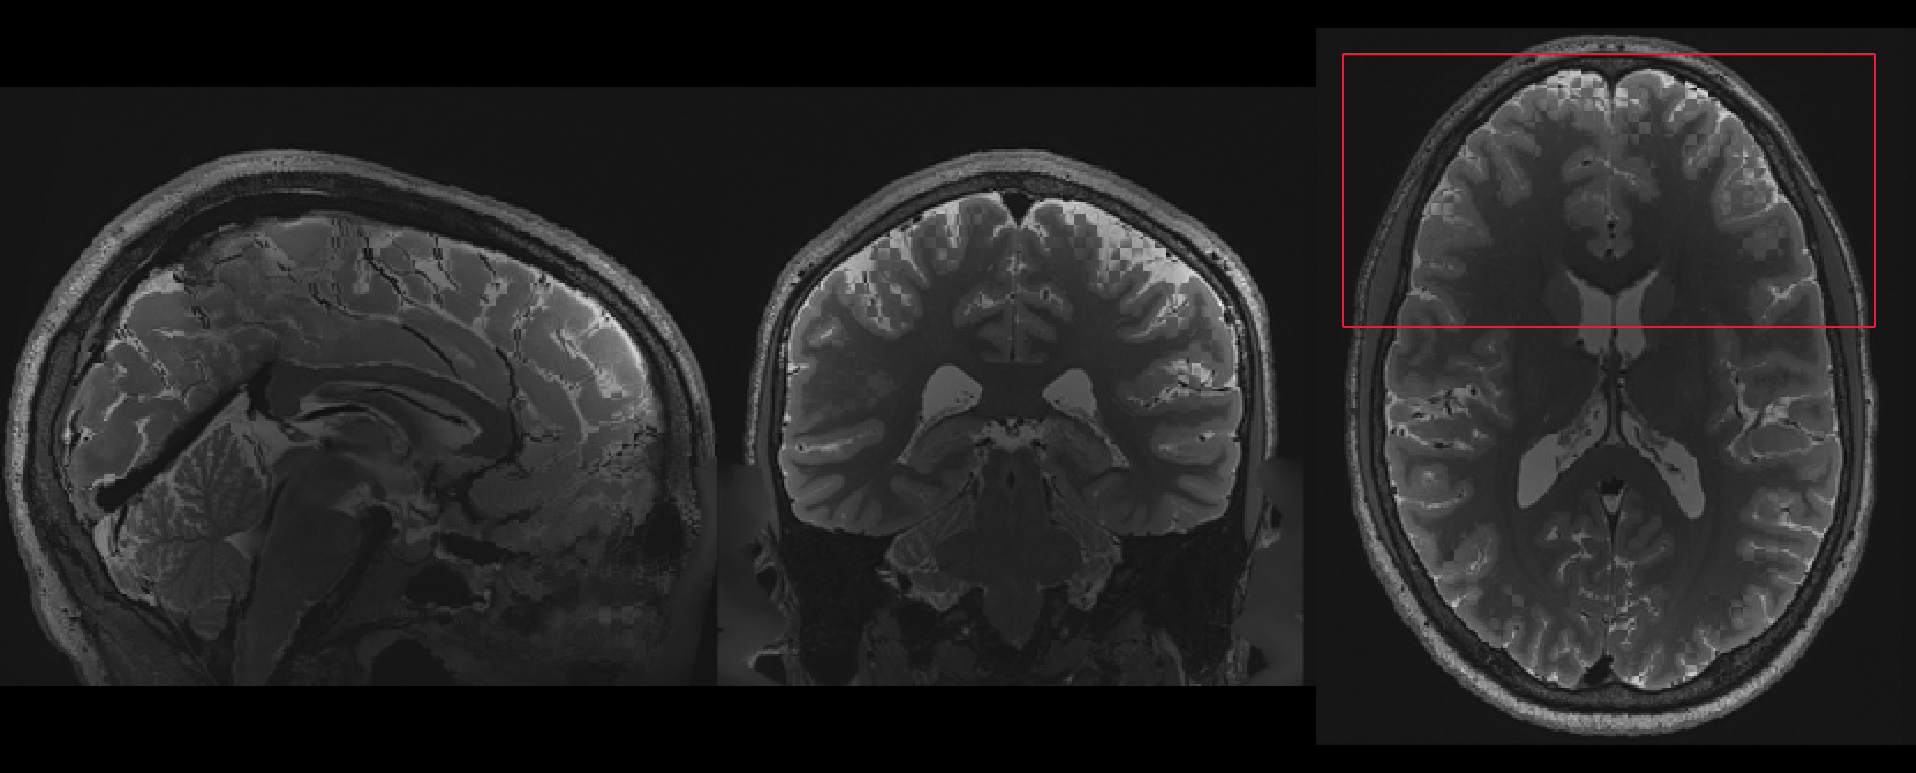
\includegraphics[width=\linewidth]{t2w_acpc_patchsize_5_copy.png}
\captionof{figure}[Differences in T2w ACPC file]{Differences in T2w ACPC file (checkerboard image). \href{https://drive.google.com/file/d/1NrNl7POyCS_SZm3an00wOLUnkmLJ_ngo/view?usp=sharing}{Link to the animated illustration of differences}.\\Figure~\ref{fig:prefreesurfer_zoom_t2w} shows the zoomed version part of the image marked by the red square. \\(Subject: 105216; Filename: T2w\_acpc\_nii.gz; Dice coeff.: 5.53*10\textsuperscript{-02} ; NRMSE: 0.0352)}
\label{fig:prefreesurfer_t2w_acpc}
\end{center}

\begin{center}
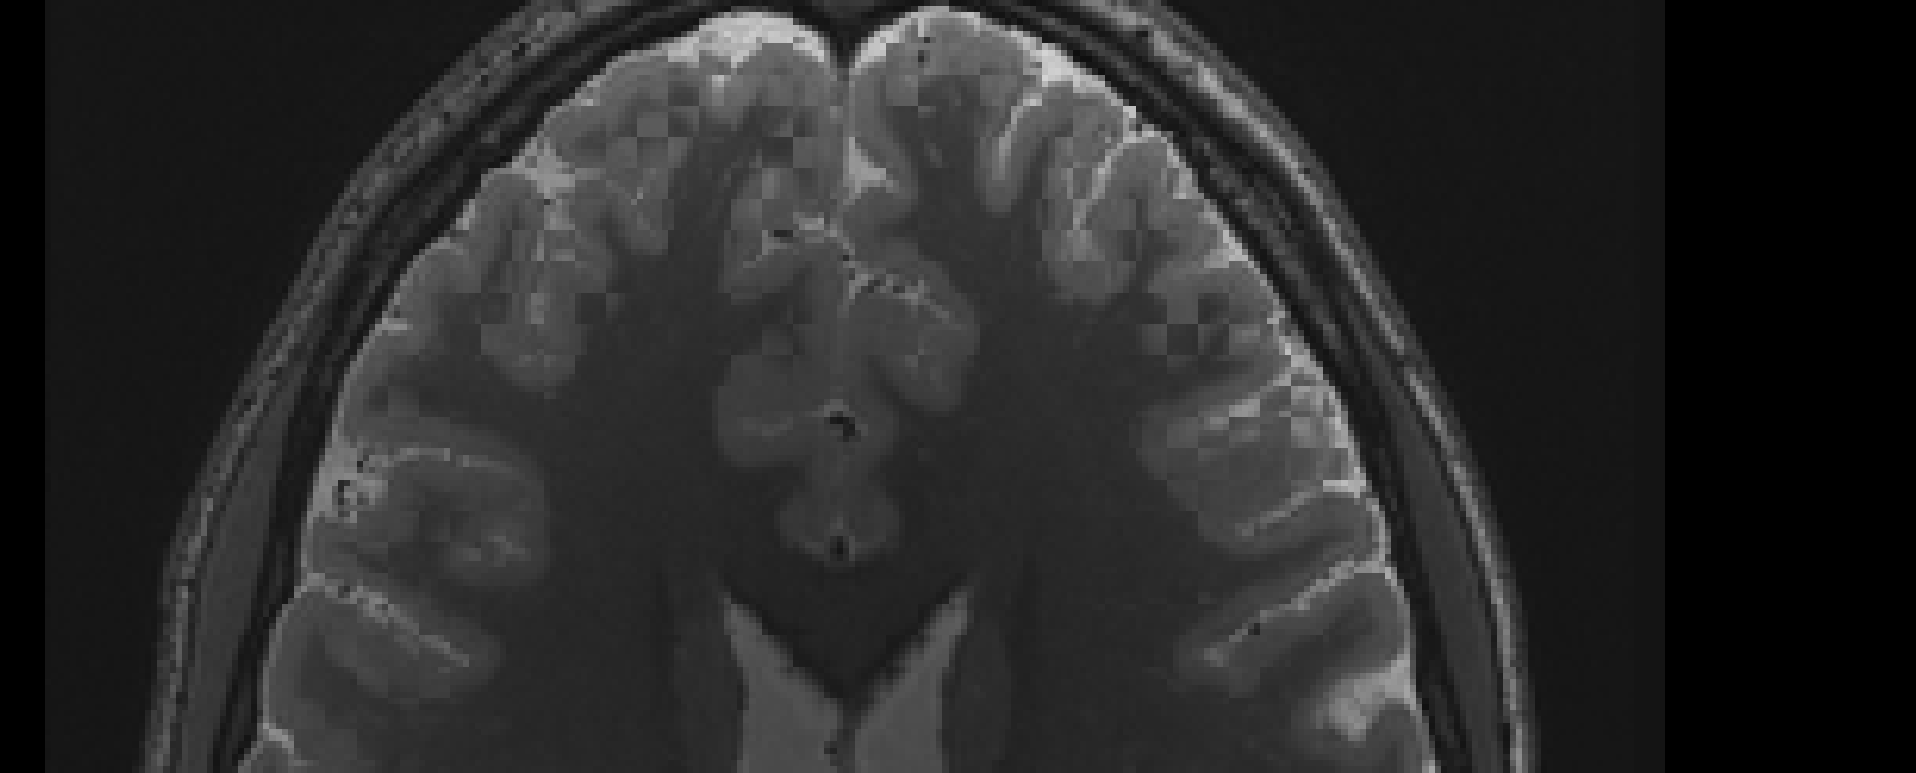
\includegraphics[width=.8\linewidth]{zoom_t2w_acpc.png}
\captionof{figure}[Zoomed in version of T2w ACPC checkerboard image]{Zoomed in version of part of checkerboard image marked with red square given in Figure~\ref{fig:prefreesurfer_t2w_acpc}}
\label{fig:prefreesurfer_zoom_t2w}
\end{center}

The visualization of the differences in T2w ACPC file given in the link above, shows that the images from two conditions are totally out of alignment. This difference is the created due to linear registration done using FLIRT (step (4), Figure \ref{fig:prefreesurfer_overview}) in PreFreeSurfer preprocessing pipeline.

Figure~\ref{fig:prefreesurfer_std_file} illustrates the differences in the ``bias\_raw.nii.gz".
This file gets created as part of bias field correction (step (10), Figure \ref{fig:prefreesurfer_overview}). The file was taken from subject ``105216". File has an NRMSE value of 0.036 and the Dice coefficient value is 0.2*10\textsuperscript{-7}. The small squares in the image shows the differences in between two conditions (CentOS6 and CentOS7).
Figure~\ref{fig:prefreesurfer_raw_file} illustrates the zoomed version of portion of checkerboard image marked with red square containing differences in Figure~\ref{fig:prefreesurfer_std_file}.
The link given below at the caption of the image contains the CentOS6 and CentOS7 files alternating in between each other.

\begin{center}
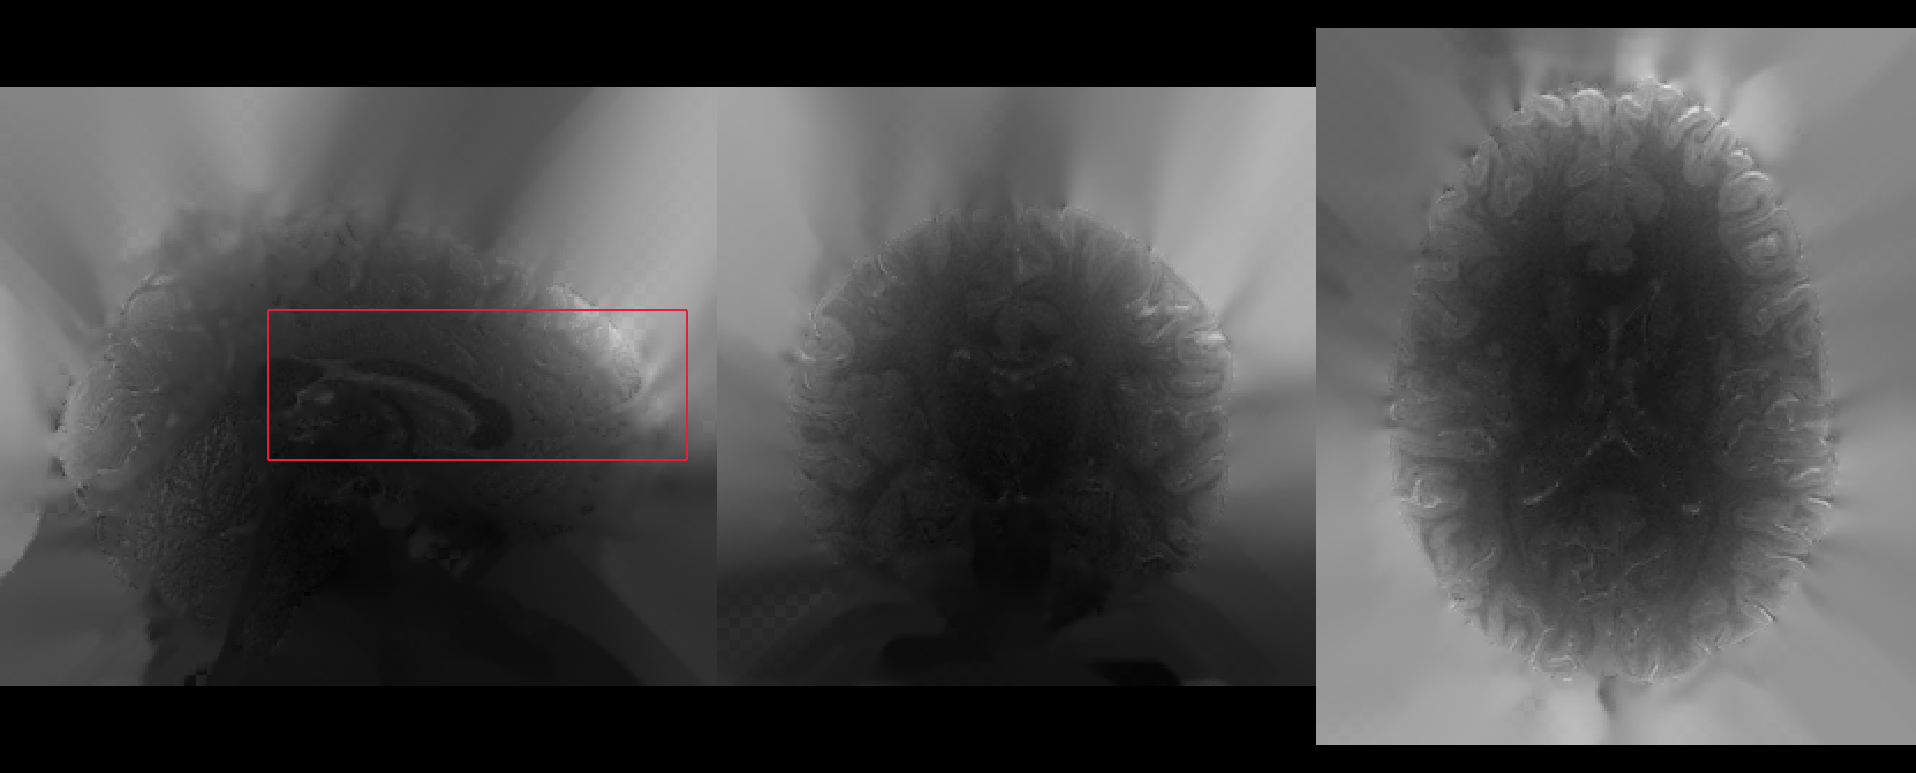
\includegraphics[width=\linewidth]{raw_bias_patchsize5_copy.png}
\captionof{figure}[Differences in bias raw file]{Differences in bias raw file (checkerboard image). \href{https://drive.google.com/file/d/1rbGR0zGPQsOPzEVkiR6NynudbfjDFLvn/view?usp=sharing}{Link to the animated illustration of differences}.\\Figure~\ref{fig:prefreesurfer_raw_file} shows the zoomed version of part of the image marked by the red square.\\(Subject: 105216; Filename: bias\_raw.nii.gz; Dice coeff.: 6.04*10\textsuperscript{-6} ; NRMSE: 0.0065)}
\label{fig:prefreesurfer_std_file}
\end{center}

\begin{center}
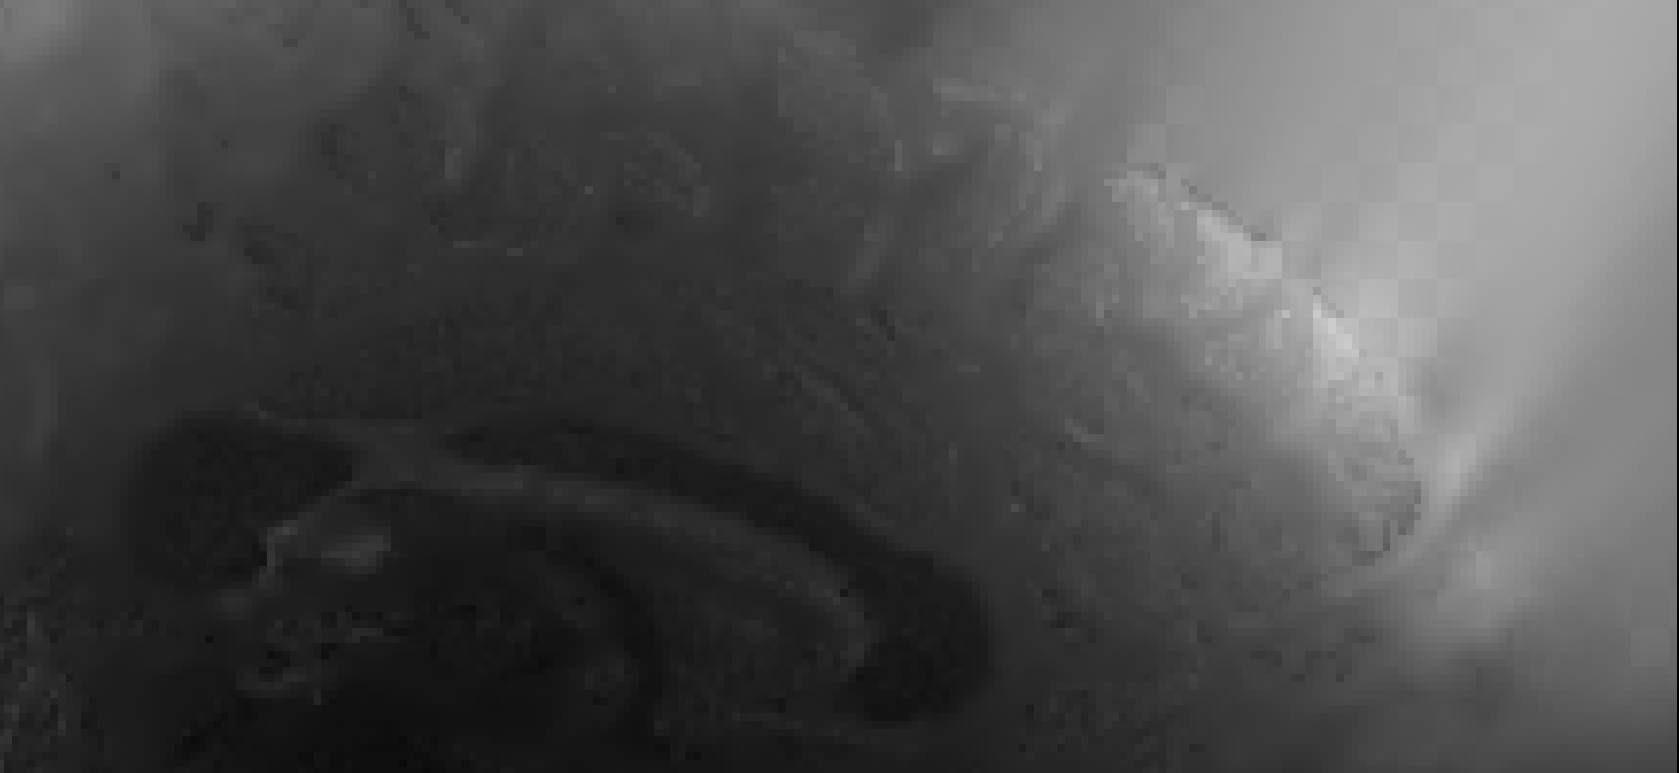
\includegraphics[width=\linewidth]{raw_bias_ps.png}
\captionof{figure}[Zoomed in bias raw file]{Zoomed in version of part of checkerboard image marked with red square given in Figure~\ref{fig:prefreesurfer_std_file}}
\label{fig:prefreesurfer_raw_file}
\end{center}

\section{FreeSurfer} \label{sec:Freesurfer}
FreeSurfer results presented in this section do not take into account the files that were found to be different in PreFreeSurfer pipeline. The number of files that have differences and which are common to all the subjects, was found to be 61 (23 .nii.gz files and 38 .mgz files).

\subsection{Global comparison}
The general findings about the differences in the output images due to the FreeSurfer processing is discussed in this section.

\begin{center}
\begin{tabular}{|l|l|l|}
\hline
\textbf{Item}      & \textbf{Nrmse} & \textbf{Dice} \\ \hline
Mean               & 0.0177    & 0.6953  \\ \hline
Median             & 0.0098    & 0.9262   \\ \hline
Standard Deviation & 0.0181     & 0.4051   \\ \hline
\end{tabular}
\captionof{table}[NRMSE \& DICE values of FreeSurfer]{NRMSE \& DICE values of FreeSurfer processing on CentOS6 and CentOS7}
\label{tab:FreeSurfer_Metic_Values}
\end{center}

Table \ref{tab:FreeSurfer_Metic_Values} contains the mean, median and standard deviation of files having differences from FreeSurfer preprocessing on CentOS6 and CentOS7. Dice Coefficient shows that out of the results we obtained from FreeSurfer processing on two conditions, there was 69\% similarity while taking the average of Dice coeffiecient of every file that we found to have a checksum difference.
\begin{center}
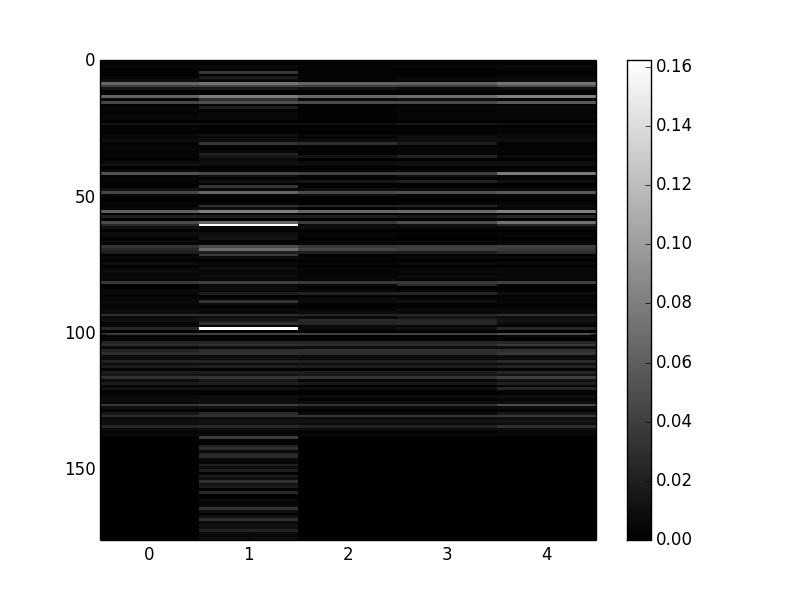
\includegraphics[width=.5\linewidth]{freesurfer-nrmse.png}%
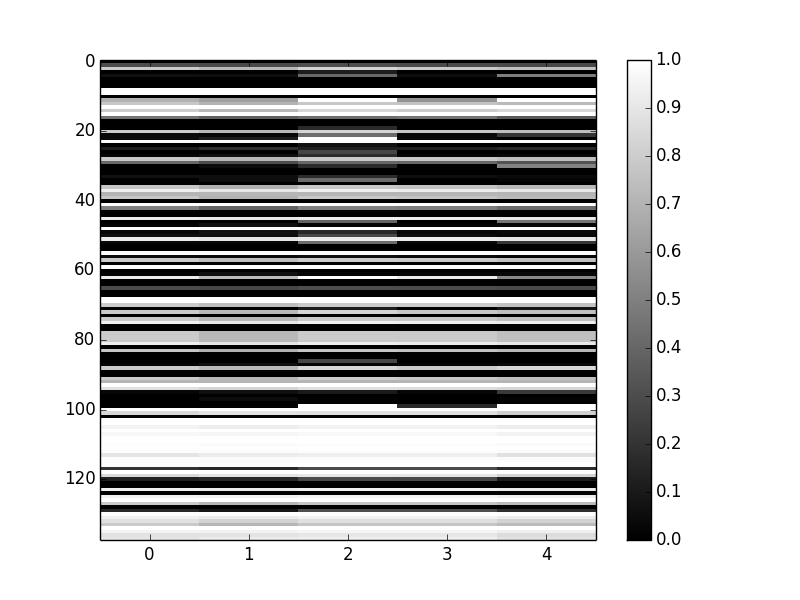
\includegraphics[width=.5\linewidth]{freesurfer-dice.png}
\captionof{figure}{FreeSurfer metric values}
\caption*{(i) NRMSE (left) (ii)Dice Coefficient (right)}
\label{fig:freesurfer_metric_values}
\end{center}

Figure \ref{fig:freesurfer_metric_values} contains the matrices showing the plotted values of NRMSE (left) and Dice Coefficient (right). Each line in the matrix corresponds to a file common to all the subjects. Each column represents a subject and each row represents the same file in 5 different subjects. The NRMSE value appears brighter if the images are dissimilar and it appears darker if the images are similar. Conversely, the Dice coefficient value appears darker if the images are dissimilar and appears brighter if the images are similar. We can also observe that the magnitude of differences varies across the files as well as the subjects.

\subsection{Comparison of specific files}
Figure~\ref{fig:freesurfer_ribbon_file} illustrates the differences in the ``ribbon.nii.gz" file. FreeSurfer pipeline produces this file in step (7) (Figure \ref{fig:freesurfer_overview}) for high resolution pial surface placement with grey matter intensity normalization and T2w exclusion of Dura and Vessels.
The file was taken from subject ``105216". The file illustrated here has an NRMSE value of 0.081 and the Dice coefficient value is 0.993. The red spots in the images shows the differences in the images in two conditions (CentOS6 and CentOS7). These localized differences are spread across the entire image.
The link given below at the caption of the image contains the visualized CentOS6 and CentOS7 files with differences, alternating in between each other.

\begin{center}
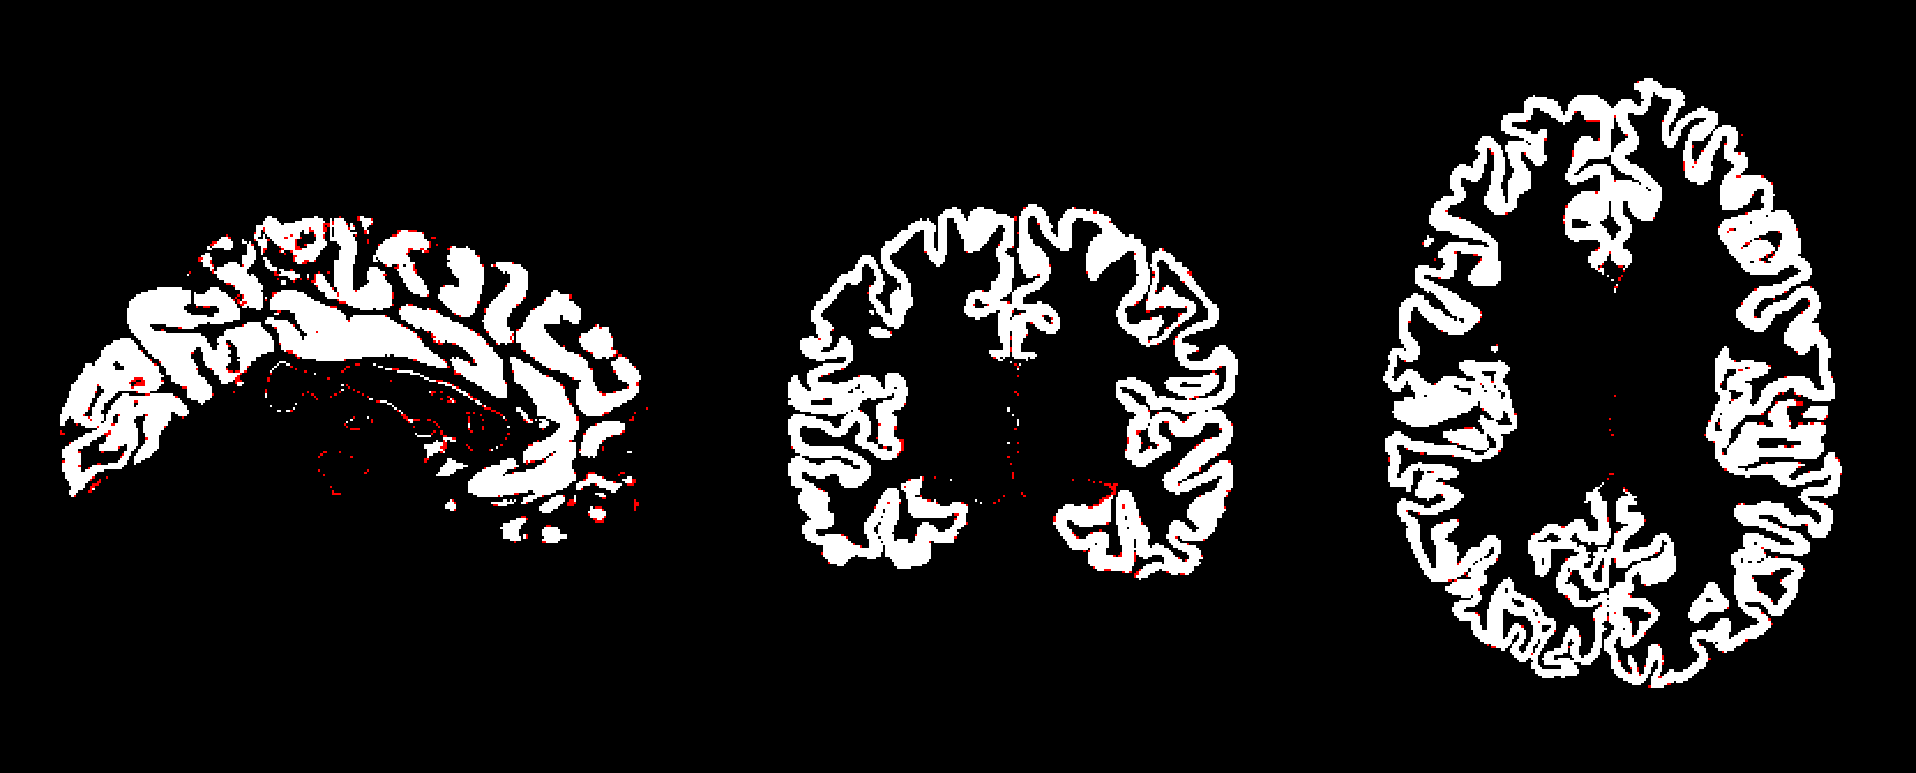
\includegraphics[width=\linewidth]{ribbon_screenshot_freesurfer.png}
\captionof{figure}[Differences in the ribbon file]{Differences in the ribbon file (Red spots in the figure shows the differences). \href{https://drive.google.com/file/d/14nQNb9qNxqgpUrl4D1P6BYplXsGpNUx_/view?usp=sharing}{Link}\\(Subject: 105216; Filename: ribbon.nii.gz; Dice coeff.: 0.993 ; NRMSE: 0.081)}
\label{fig:freesurfer_ribbon_file}
\end{center}

Figure~\ref{fig:freesurfer_aseg_file} illustrates the differences in the ``aseg.hires.mgz" file. This file gets created under mri directory inside T1w file directory. The file was taken from subject ``105216". The file illustrated here has an NRMSE value of 0.010, and the Dice coefficient value is 0.987. The bright spots in the image shows the difference in the images in between two conditions (CentOS6 and CentOS7). These localized images are spread across the image. This image is the result of segmentation which is done for identifying and segmenting the smaller structures inside the brain. Each color represents a different structure and, we can find important differences in all structures. The link given below at the caption of the image contains the visualized CentOS6 and CentOS7 files with differences, alternating in between each other.

\begin{center}
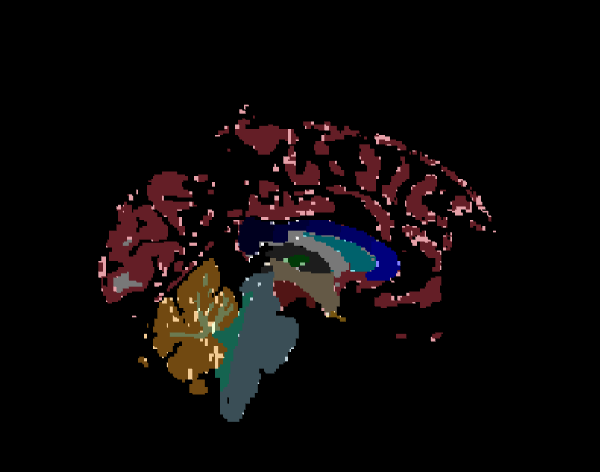
\includegraphics[width=.5\linewidth]{aseg-bright-1.png}%
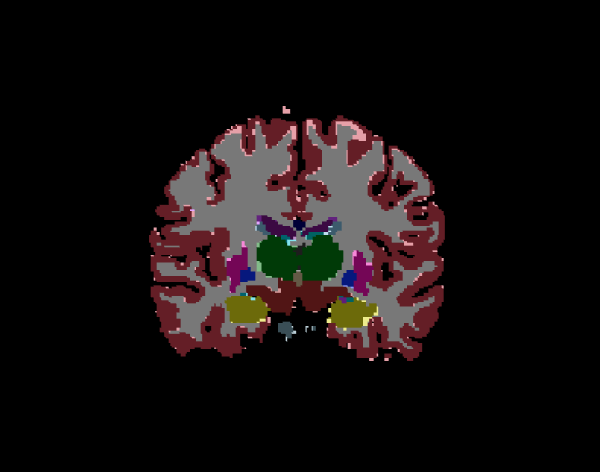
\includegraphics[width=.5\linewidth]{aseg-bright-2.png}
\captionof{figure}[Differences in aseg hires file]{Differences in aseg hires file (Bright spots in the figure shows the differences). \href{https://drive.google.com/file/d/1WUwWp5muXvotbMQqTqR5LcMyncH1ET3P/view?usp=sharing}{Link}\\(Subject: 105216; Filename: aseg.hires.mgz; Dice coeff.: 0.987 ; NRMSE: 0.010)}
\label{fig:freesurfer_aseg_file}
\end{center}

Figure~\ref{fig:freesurfer_wm_file} illustrates the differences in the ``wm.hires.nii.gz" file. This file also gets created after FreeSurfer processing inside mri folder under the T1w directory. The file was taken from subject ``105216". The file illustrated here has an NRMSE value of 0.074 and the Dice coefficient value is 0.994. The red spots in the image shows the differences in between two conditions (CentOS6 and CentOS7). We can observe that the localized differences are spread throughout the image. The link given below at the caption of the image contains the visualized CentOS6 and CentOS7 files with differences, alternating in between each other.

\begin{center}
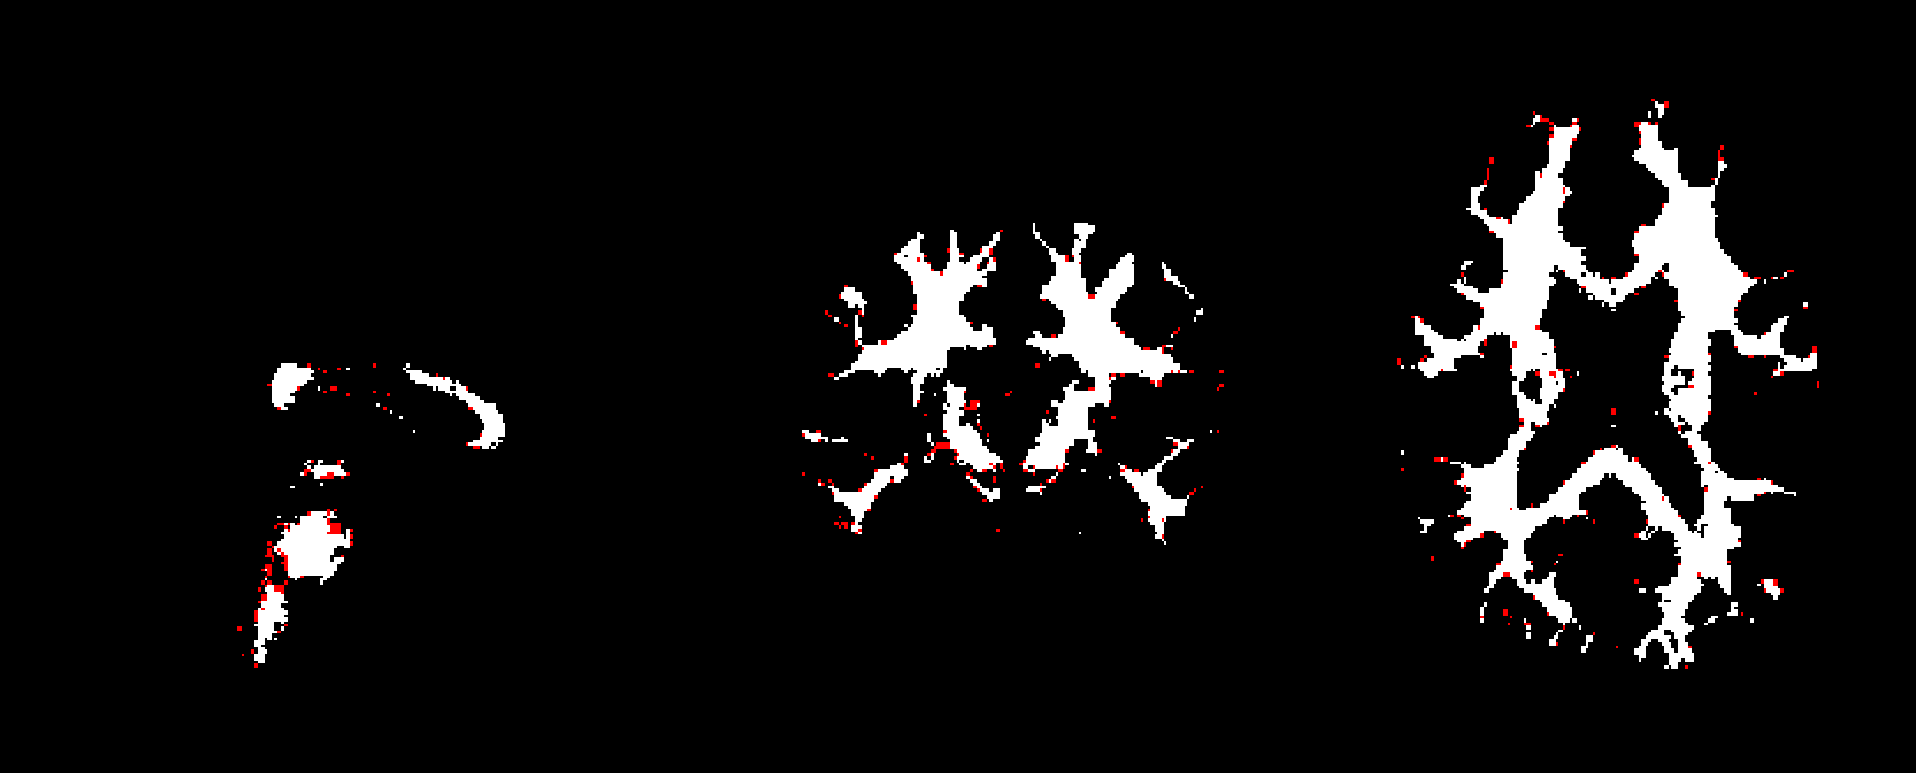
\includegraphics[width=\linewidth]{wm-red-white.png}
\captionof{figure}[Differences in WM hire file]{Differences in WM hire file (Red spots in the image shows the differences). \href{https://drive.google.com/file/d/1i6WpH6Le5xry4j-RtRZxt0_NP3Ulm5AT/view?usp=sharing}{Link}\\(Subject: 105216; Filename: wm.hires.nii.gz; Dice coeff.: 0.994 ; NRMSE: 0.074)}
\label{fig:freesurfer_wm_file}
\end{center}

\section{PostFreeSurfer}\label{sec:Postfreesurfer}
25 (.nii.gz) were found to have inter-OS differences after PostFreeSurfer processing. These files are created as part of PostFreeSurfer processing alone, and they are common to all the five subjects.

\subsection{Global comparison}
The general findings about the differences in the output images due to the PostFreeSurfer processing is discussed in this section.

\begin{center}
\begin{tabular}{|l|l|l|}
\hline
\textbf{Item}      & \textbf{Nrmse} & \textbf{Dice} \\ \hline
Mean               & 0.0347     & 0.6768   \\ \hline
Median             & 0.0386    & 0.9829   \\ \hline
Standard Deviation & 0.0254    & 0.4584   \\ \hline
\end{tabular}
  \captionof{table}[NRMSE \& DICE values of PostFreeSurfer]{NRMSE \& DICE values of PostFreeSurfer processing on CentOS6 and CentOS7}
\label{tab:PostFreeSurfer_Metic_Values}
\end{center}

Table \ref{tab:PostFreeSurfer_Metic_Values} contains the mean, median and standard deviation values of files having differences from PostFreeSurfer pipeline on CentOS6 and CentOS7 operating systems. Dice Coefficient shows that out of the results we obtained from PostFreeSurfer processing on two conditions, there was 67\% similarity while taking the average of Dice coefficient of every file that we found to have a checksum difference.

\begin{center}
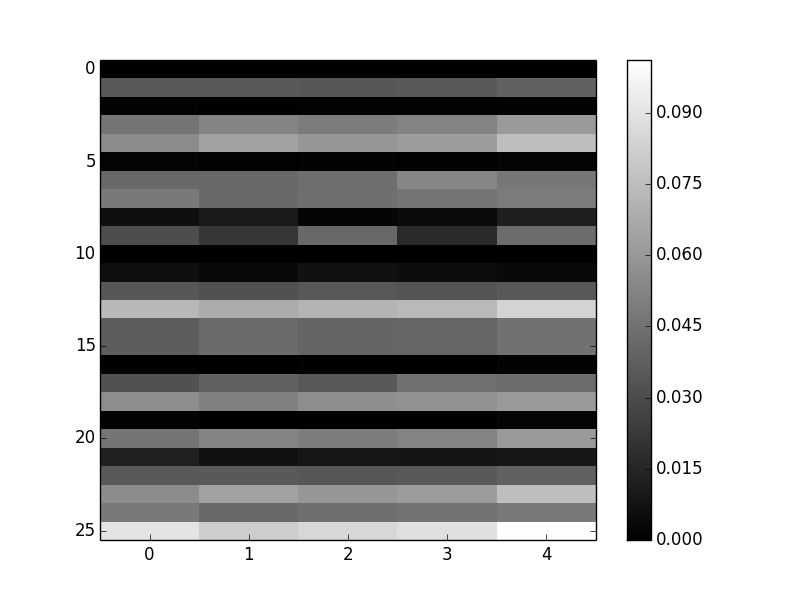
\includegraphics[width=.5\linewidth]{postfreesurfer-nrmse.png}%
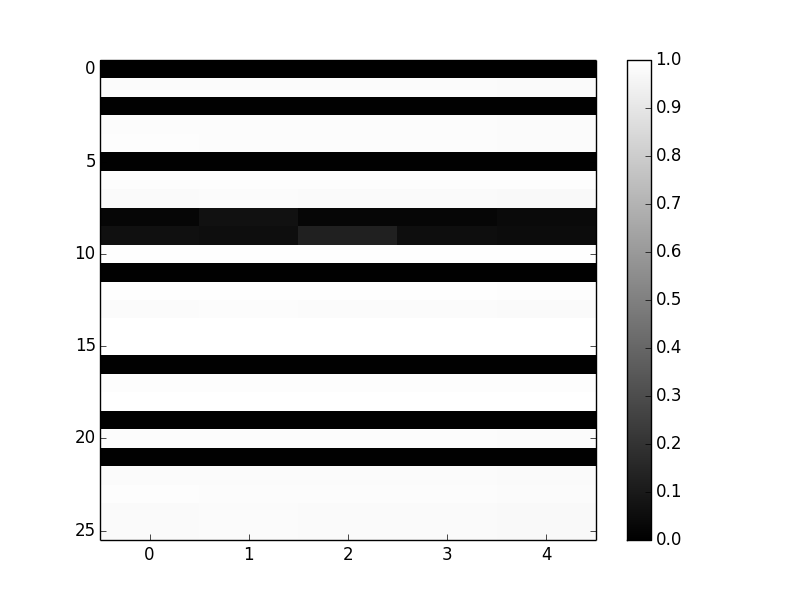
\includegraphics[width=.5\linewidth]{postfreesurfer-dice.png}
\captionof{figure}{PostFreeSurfer metric values}
\caption*{(i) NRMSE (left) (ii)Dice Coefficient (right)}
\label{fig:postfreesurfer_metric_values}
\end{center}

Figure \ref{fig:postfreesurfer_metric_values} contains the matrices showing the plotted values of NRMSE (left) and Dice Coefficient (right). Each line in the matrix corresponds to a file common to all the subjects. Each column represents a subject and each row represents the same file in 5 different subjects. The files are sorted according to the modification time. The NRMSE value appears brighter if the images are dissimilar and it appears darker if the images are similar. Conversely, the Dice coefficient value appears darker if the images are dissimilar and appears brighter if the images are similar. We can also observe that the magnitude of differences varies across the files as well as the subjects.

\subsection{Comparison of specific files}
Figure~\ref{fig:postfreesurfer_high_nrmse} illustrates the differences in the ``aparc.a2009s+aseg.nii.gz" file. The file was taken from MNINonLinear directory in subject ``101410". The file illustrated here has an NRMSE value of 0.101 and the Dice coefficient value is 0.97. The bright spots in the image shows the differences in between two conditions (CentOS6 and CentOS7). We can observe the localized differences spread across the images. The link given below at the caption of the image contains the visualized CentOS6 and CentOS7 files with differences, alternating in between each other.

\begin{center}
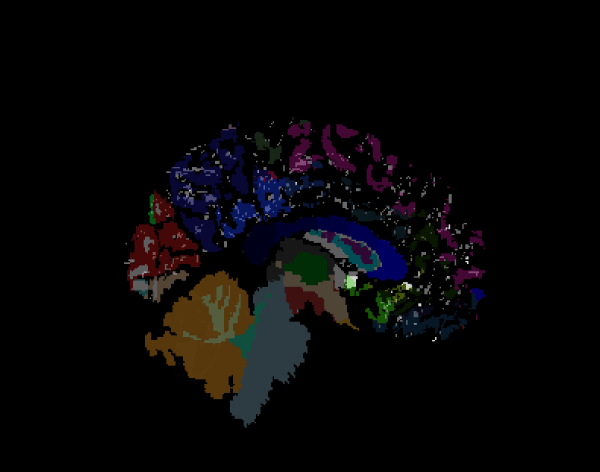
\includegraphics[width=.5\linewidth]{a20091.png}%
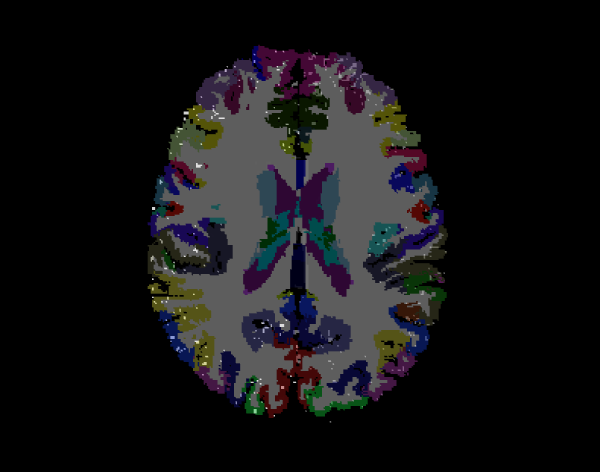
\includegraphics[width=.5\linewidth]{a20092.png}
  \captionof{figure}[Differences in aparc.a2009s+aseg file]{Differences in aparc.a2009s+aseg file (Bright spots in the image indicates the differences). \href{https://drive.google.com/file/d/1eeofWaPyk-A2pQd6LlieQwbMYVOrfeI3/view?usp=sharing}{Link}\\(Subject: 101410; Filename: aparc.a2009s+aseg.nii.gz; Dice coeff.: 0.97 ; NRMSE: 0.101)}
\label{fig:postfreesurfer_high_nrmse}
\end{center}

Figure~\ref{fig:postfreesurfer_ribbon_file} illustrates the differences in the ``ribbon.nii.gz" file. PostFreeSurfer creates this file as a part of generation of cortical ribbon volume (step (3) - Figure \ref{fig:postfreesurfer_overview}). The file was taken from T1w directory in subject ``105216". The file illustrated here has an NRMSE value of 0.038 and the Dice coefficient value is 0.995. The bright spots in the image shows the difference in the image in between two conditions (CentOS6 and CentOS7). We can observe the localized differences spread across the images. The link given below at the caption of the image contains the visualized CentOS6 and CentOS7 files with differences, alternating in between each other.

\begin{center}

\includegraphics[width=.5\linewidth]{ribbon_postfreesurfer2.png}%
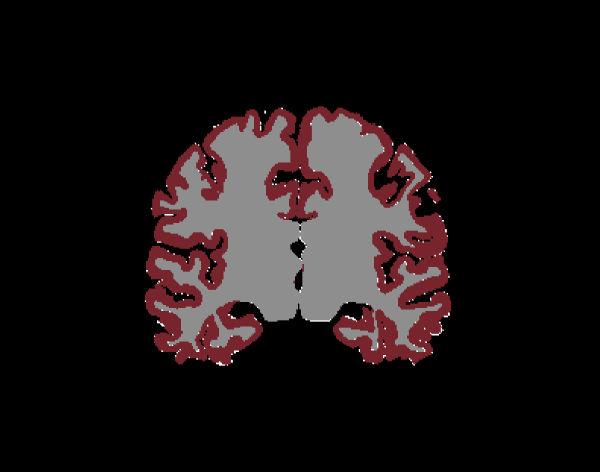
\includegraphics[width=.5\linewidth]{ribbon_postfreesurfer.png}
\captionof{figure}[Differences in the T1w Ribbon file]{Differences in the T1w Ribbon file (Bright spots in the image shows the differences). \href{https://drive.google.com/file/d/1KGEvLP4bltu5k6m9tttoTuhehaH3ldGk/view?usp=sharing}{Link}\\(Subject: 105216; Filename: ribbon.nii.gz; Dice coeff.: 0.995 ; NRMSE: 0.038)}
\label{fig:postfreesurfer_ribbon_file}
\end{center}

Figure~\ref{fig:postfreesurfer_aparc_file} illustrates the differences in the ``aparc+aseg.nii.gz" file. The file was taken from MNINonLinear directory from subject ``101006". The file illustrated here has an NRMSE value of 0.073 and the Dice coefficient value is 0.98. The bright spots in the image shows the difference in the image in between two conditions (CentOS 6 and CentOS7). We can find localized differences spread across the images. The link given below at the caption of the image contains the visualized CentOS6 and CentOS7 files with differences, alternating in between each other.

\begin{center}

\includegraphics[width=.5\linewidth]{aparc_aseg1.png}%
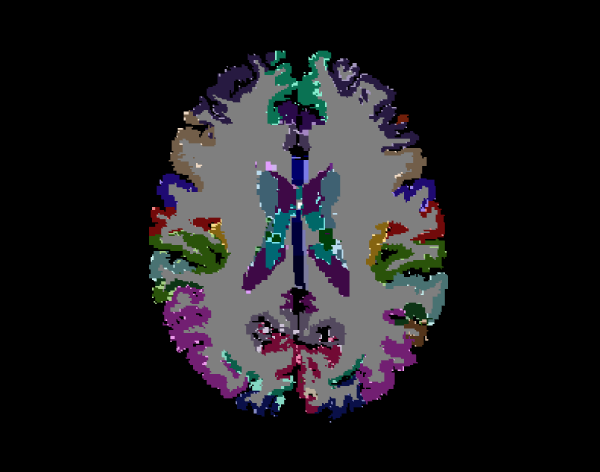
\includegraphics[width=.5\linewidth]{aparc_aseg2.png}%
\captionof{figure}[Differences in the segmentation file]{Differences in the segmentation file (Bright spots in the image indicates the differences). \href{https://drive.google.com/file/d/1_ZyAtveS1oVle8tAXeKsp1_4KdS2MVoB/view?usp=sharing}{Link}\\(Subject: 101006; Filename: aparc+aseg.nii.gz; Dice coeff.: 0.98 ; NRMSE: 0.073)}
\label{fig:postfreesurfer_aparc_file}
\end{center}

\section{fMRIVolume}\label{sec:fMRI}
1152 files were found to have inter-OS differences after fMRIVolume processing which were common to all subjects.
\subsection{Global comparison}
The general findings about the differences in the output images due to the fMRIVolume processing is discussed in this section.

\begin{center}
\begin{tabular}{|l|l|l|}
\hline
\textbf{Item}      & \textbf{Nrmse}  & \textbf{Dice} \\ \hline
Mean               & 0.0160    & 0.5605   \\ \hline
Median             & 0.0090     & 0.7511   \\ \hline
Standard Deviation & 0.0196     & 0.3769   \\ \hline
\end{tabular}
  \captionof{table}[NRMSE \& DICE values of fMRIVolume]{NRMSE \& DICE values of fMRIVolume processing on CentOS6 and CentOS7}
\label{tab:fMRIVolume_Metric_Values}
\end{center}

Table \ref{tab:fMRIVolume_Metric_Values} contains the mean, median and standard deviation of the files having differences produced by the fMRIVolume pipeline on CentOS6 and CentOS7 operating systems. Dice Coefficient shows that out of the results we obtained from fMRIVolume processing on two conditions, there was 56\% similarity while taking the average of Dice coefficient of every file that we found to have a checksum difference.

\begin{center}
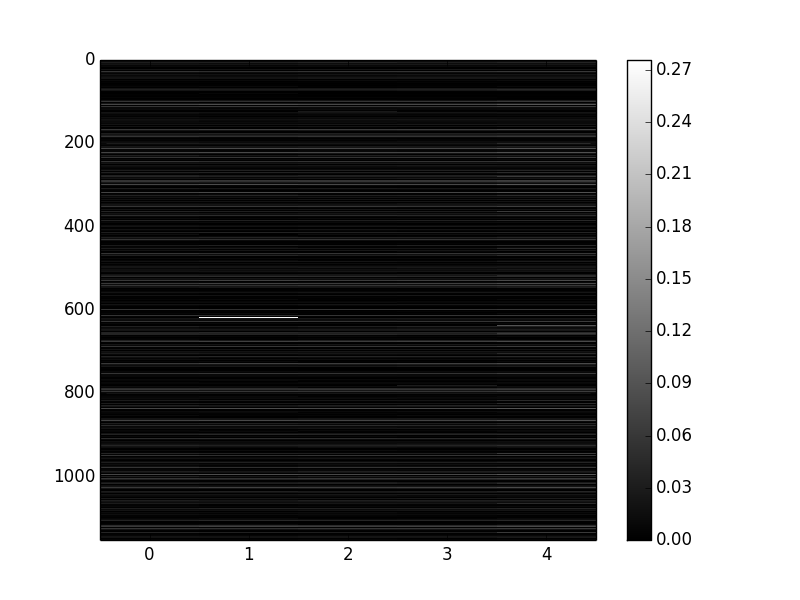
\includegraphics[width=.5\linewidth]{fmri_NRMSE.png}%
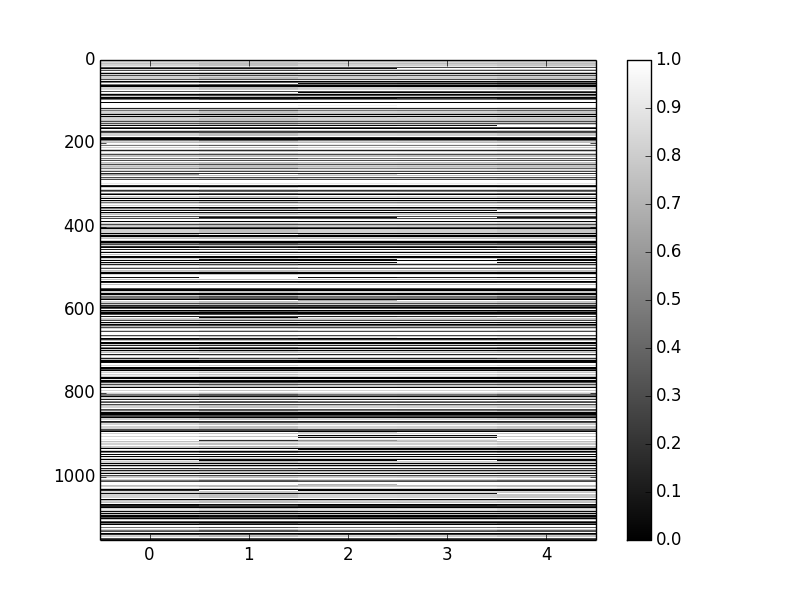
\includegraphics[width=.5\linewidth]{fmri_DICE.png}
\captionof{figure}{fMRIVolume metric values}
\caption*{(i) NRMSE (left) (ii)Dice Coefficient (right)}
\label{fig:fMRI_metric_values}
\end{center}

Figure \ref{fig:fMRI_metric_values} contains the matrices showing the plotted values of NRMSE (left) and Dice Coefficient (right) with respect to the files having differences from the fMRIVolume pipeline preprocessing. Each line in the matrix corresponds to a file common to all the subjects. Each column represents a subject and each row represents the same file in 5 different subjects. The files are sorted according to their modification time. The NRMSE value appears brighter if the images are dissimilar and it appears darker if the images are similar. Conversely, the Dice coefficient value appears darker if the images are dissimilar and appears brighter if the images are similar. We can also observe that the magnitude of differences varies across the files as well as the subjects.

\subsection{Comparison of specific files}
Figure~\ref{fig:allgrey_matter} illustrates the differences in the ``AllGreyMatter.nii.gz" file. This file gets created at step (5) (Figure \ref{fig:fMRIVolume_overview}), with the use of FLIRT, BBR cost function and FreeSurfer's BBRegister. The file was taken from the ComputeSpinEchoBiasField directory in subject ``101006". The file illustrated here has an NRMSE value of 0.074 and the Dice coefficient value is 0.99. The red spots in the image shows the differences between the conditions (CentOS 6 and CentOS7). The localized differences are spread across the image. The link given below at the caption of the image contains the visualized CentOS6 and CentOS7 files with differences, alternating in between each other.

\begin{center}
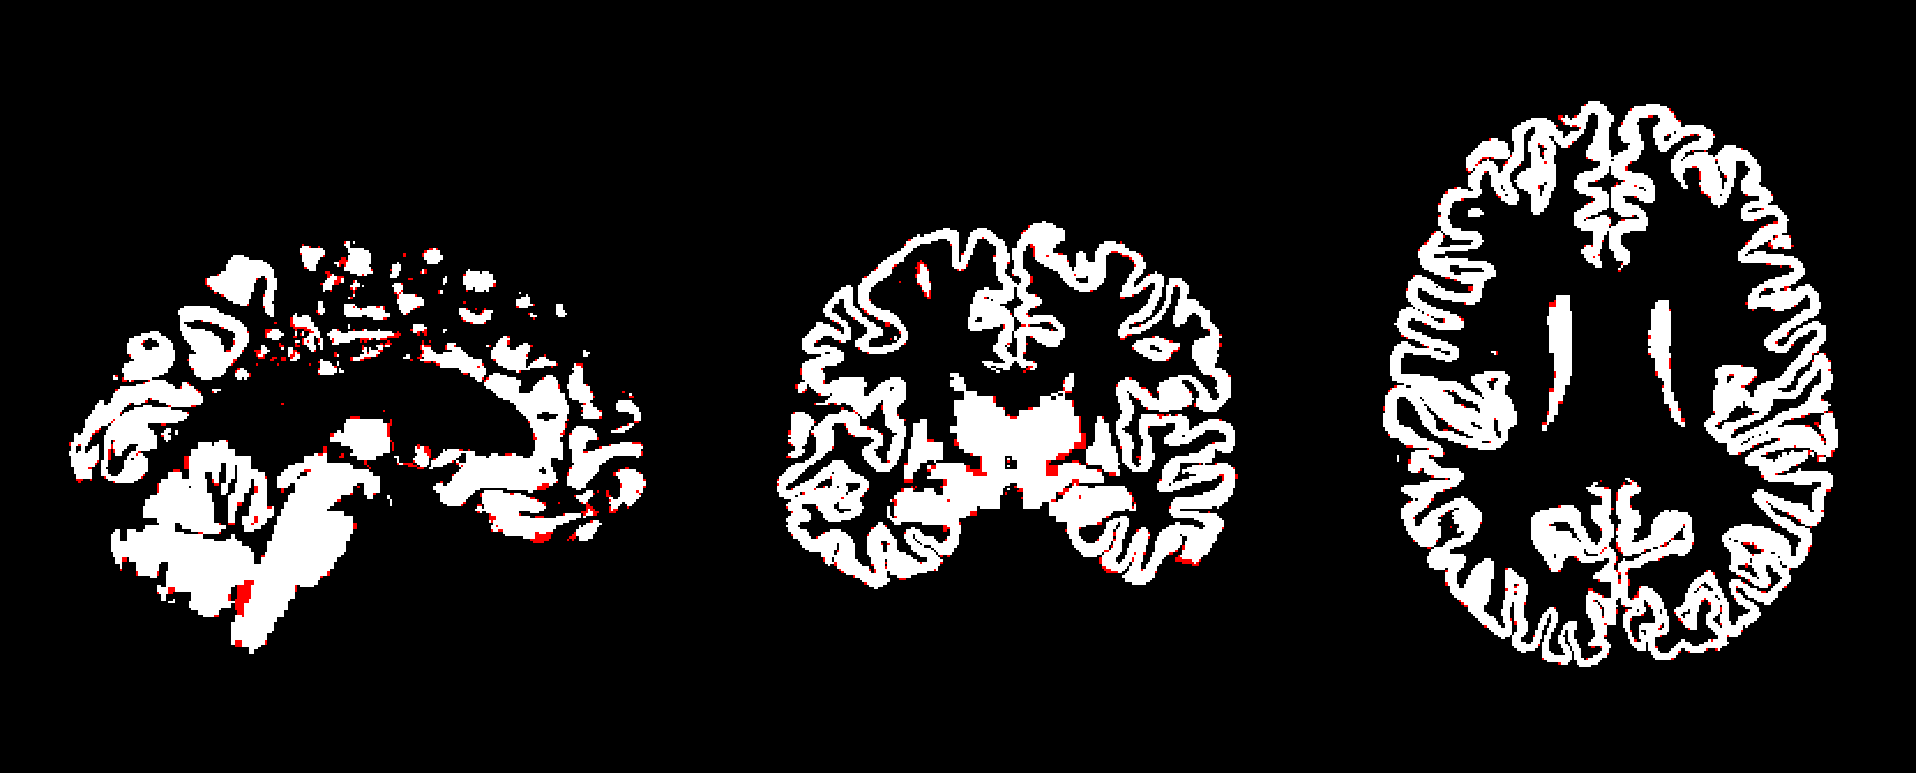
\includegraphics[width=\linewidth]{all-grey-matter.png}
\captionof{figure}[Differences in all grey matter file]{Differences in all grey matter file (Red spots in the image indicates the differences). \href{https://drive.google.com/file/d/1dzpyMalJ6_ox8jLedKvhKrP2ew7C7N-r/view?usp=sharing}{Link}\\{(Subject: 101006; Filename: AllGreyMatter.nii.gz; Dice coeff.; 0.99; NRMSE; .074)}}
\label{fig:allgrey_matter}
\end{center}

Figure~\ref{fig:tfMRI_mask_file} illustrates the differences in the ``tfMRI\_MOTOR\_LR\_mc\_mask.nii.gz" file. This file is created as part of motion correction in fMRIVolume pipeline (step (3), Figure \ref{fig:fMRIVolume_overview}). The image on the left is the output from CentOS6 and the image on the right is the output from CentOS7. The files are taken from MotionCorrection directory in subject ``101006". The files illustrated here has an NRMSE value of 0.275 and the Dice coefficient value is 0.002. While comparing the images, we can find the differences visually.
The link given below at the caption of the image contains the visualized CentOS6 and CentOS7 files with differences, alternating in between each other.

\begin{center}

\includegraphics[width=.5\linewidth]{tfMRI_MOTOR_LR_mc_mask_centos6.png}%
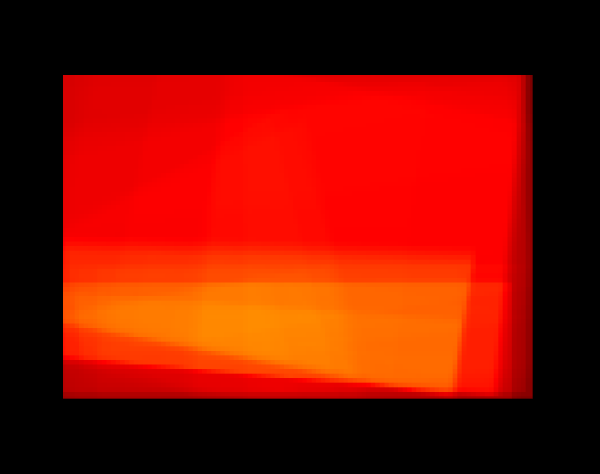
\includegraphics[width=.5\linewidth]{tfMRI_MOTOR_LR_mc_mask_centos7.png}
\captionof{figure}[Differences in tfMRI Motor MC Mask file]{Differences in tfMRI Motor MC Mask file. \href{https://drive.google.com/file/d/1_XpZnroleOlJmkvXHZA84iknT5UxtO14/view?usp=sharing}{Link}\\(Subject: 105216; Filename: tfMRI\_MOTOR\_LR\_mc\_mask.nii.gz (CentOS6 on left, CentOS7 on right); Dice coeff.; 0.0002; NRMSE; 0.275)}
\label{fig:tfMRI_mask_file}
\end{center}

Figure~\ref{fig:scout_gdc_file} illustrates the differences in the ``Scout\_gdc\_undistorted2T1w.nii.gz" file. This file gets created at step (5) (Figure \ref{fig:fMRIVolume_overview}), with the use of FLIRT, BBR cost function and FreeSurfer's BBRegister. The files are taken from the directory DistortionCorrectionAndEPIToT1wReg\_FLIRTBBRAndFreeSurferBBRbased in subject ``101410". The files illustrated here have an NRMSE value of 0.010 and the Dice coefficient value is 0.778. The small squares in the image indicates the differences. Figure~\ref{fig:scout_zoom} shows the zoomed in version of portion of the checkerboard image marked by red square in Figure~\ref{fig:scout_gdc_file}. The link given below at the caption of the image contains the visualized CentOS6 and CentOS7 files with differences, alternating in between each other.

\begin{center}
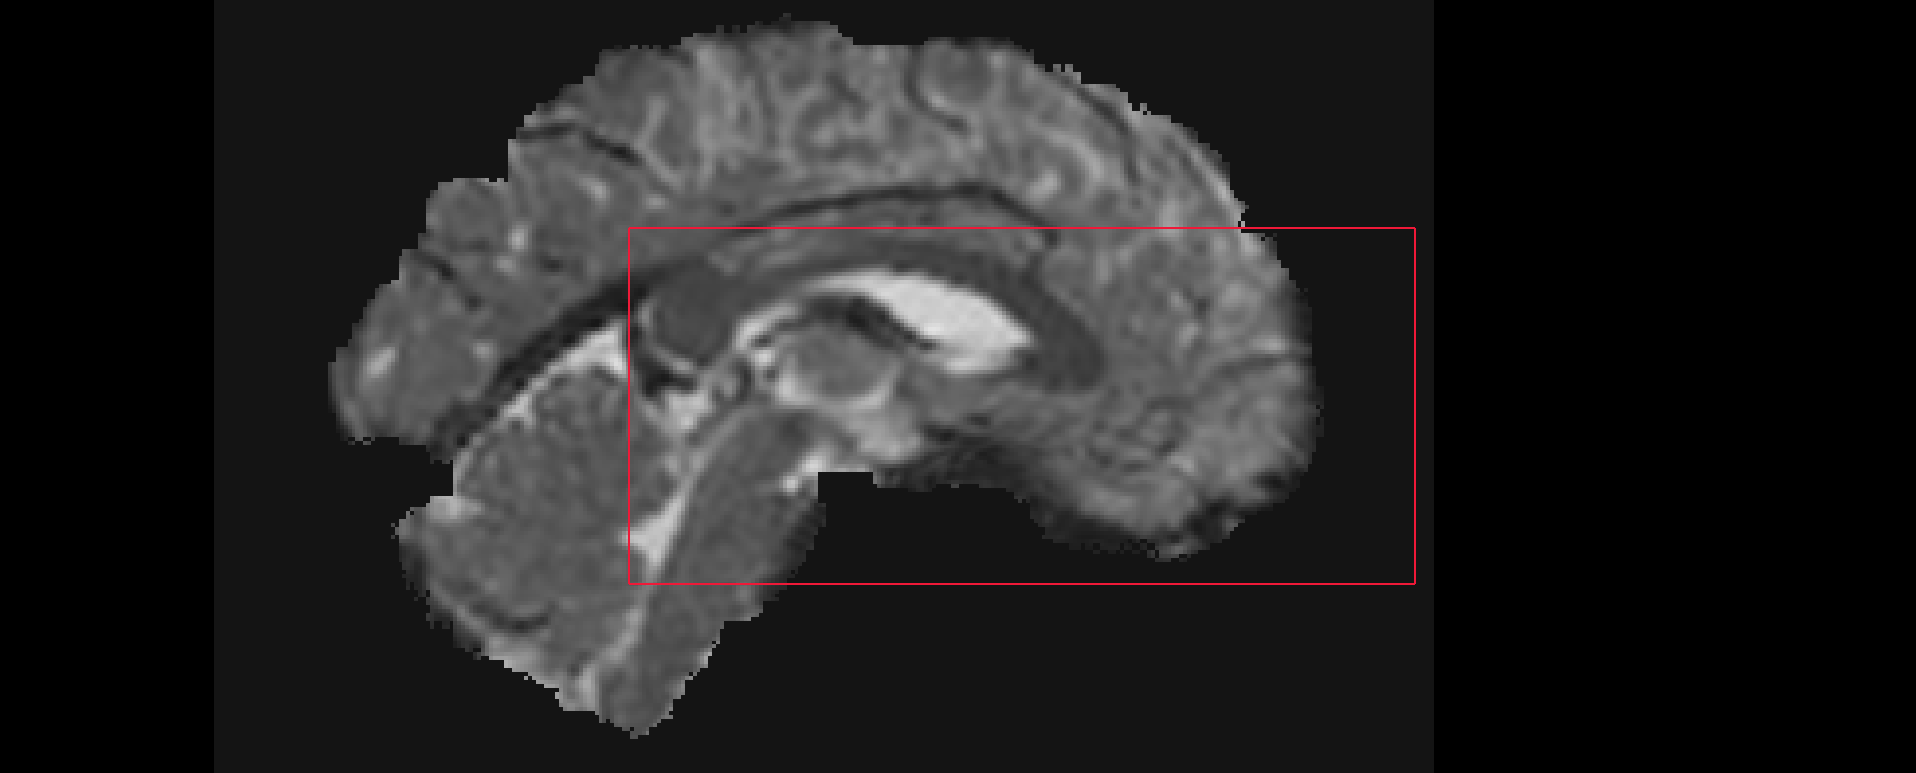
\includegraphics[width=\linewidth]{scout_patchsize2-1-copy.png}%
%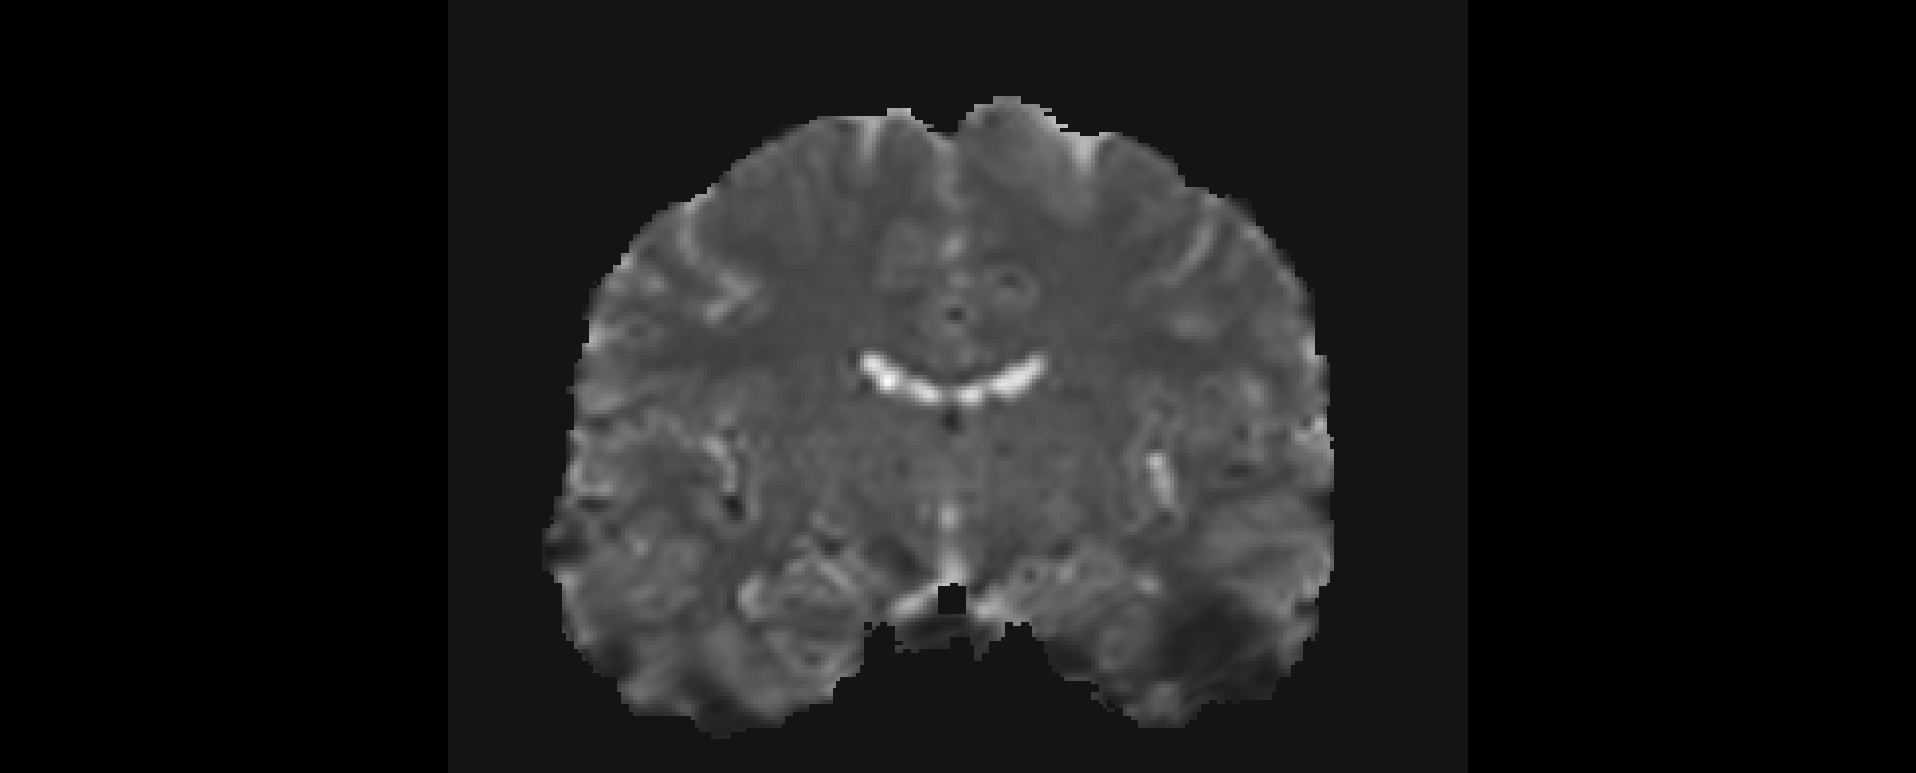
\includegraphics[width=.33\linewidth]{scout_patchsize2-2.png}%
%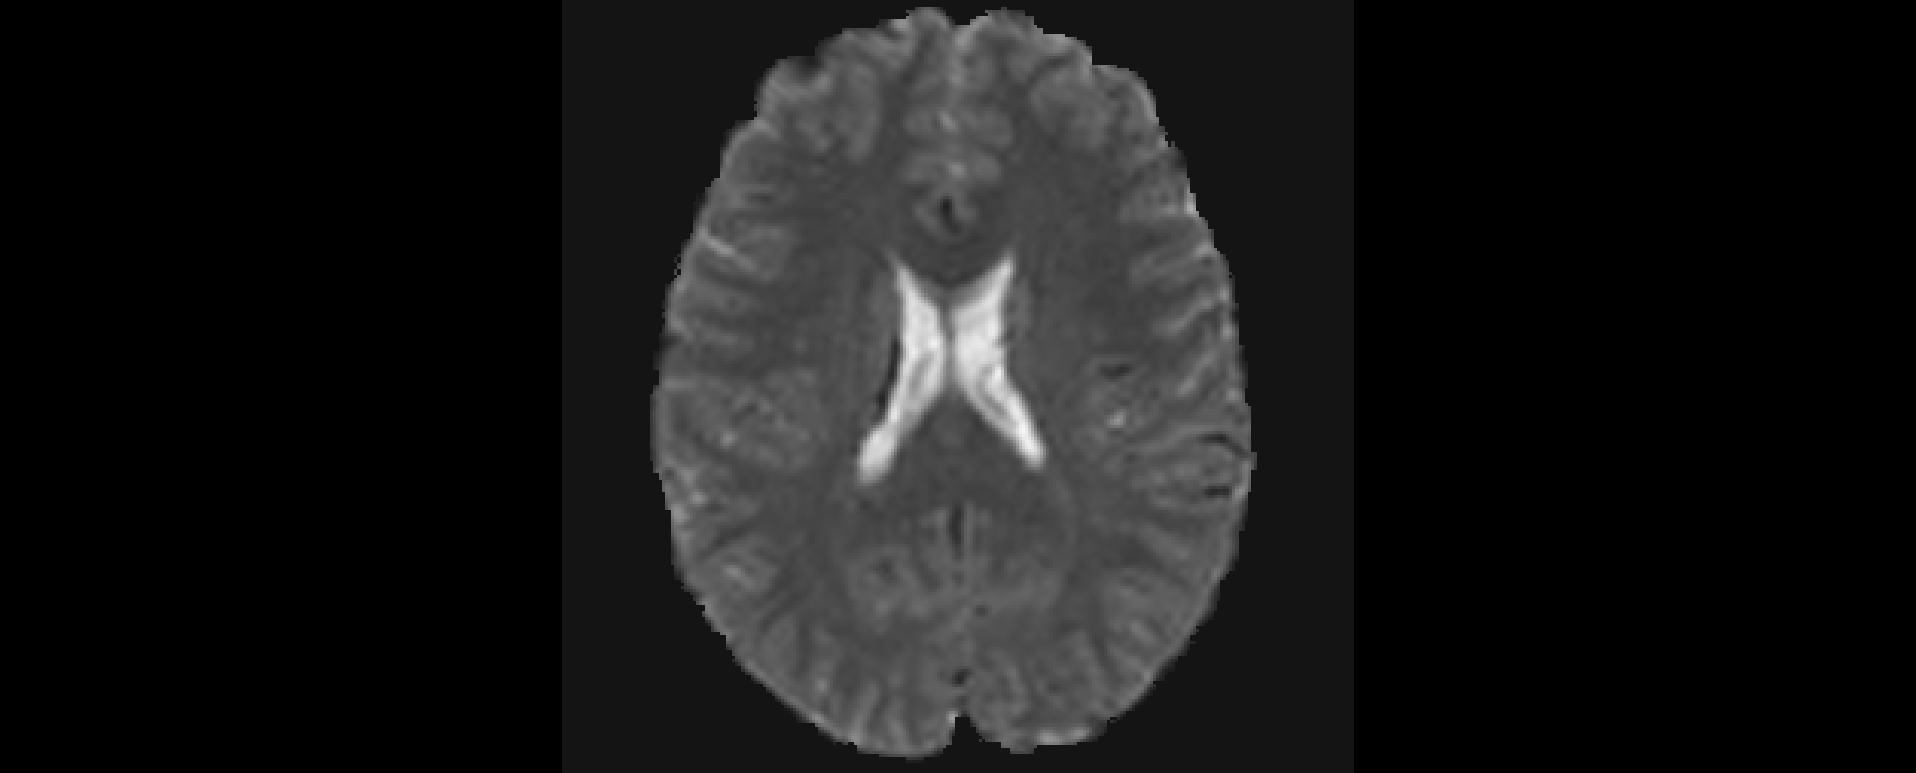
\includegraphics[width=.33\linewidth]{scout_patchsize2-3.png}
\captionof{figure}[Differences in the Scout\_gdc\_undistorted2T1w file]{Differences in the Scout\_gdc\_undistorted2T1w file (checkerboard image). \href{https://drive.google.com/file/d/1iRP6jVMKbGBLjLdEi3l5j4Q8Pngp5Nln/view?usp=sharing}{Link to the animated illustration of differences}.\\Figure~\ref{fig:scout_zoom} shows the zoomed version part of the image marked by the red square.\\(Subject: 101410; Filename: Scout\_gdc\_undistorted2T1w.nii.gz ; Dice coeff.; 0.778; NRMSE; 0.010)}
\label{fig:scout_gdc_file}
\end{center}

\begin{center}
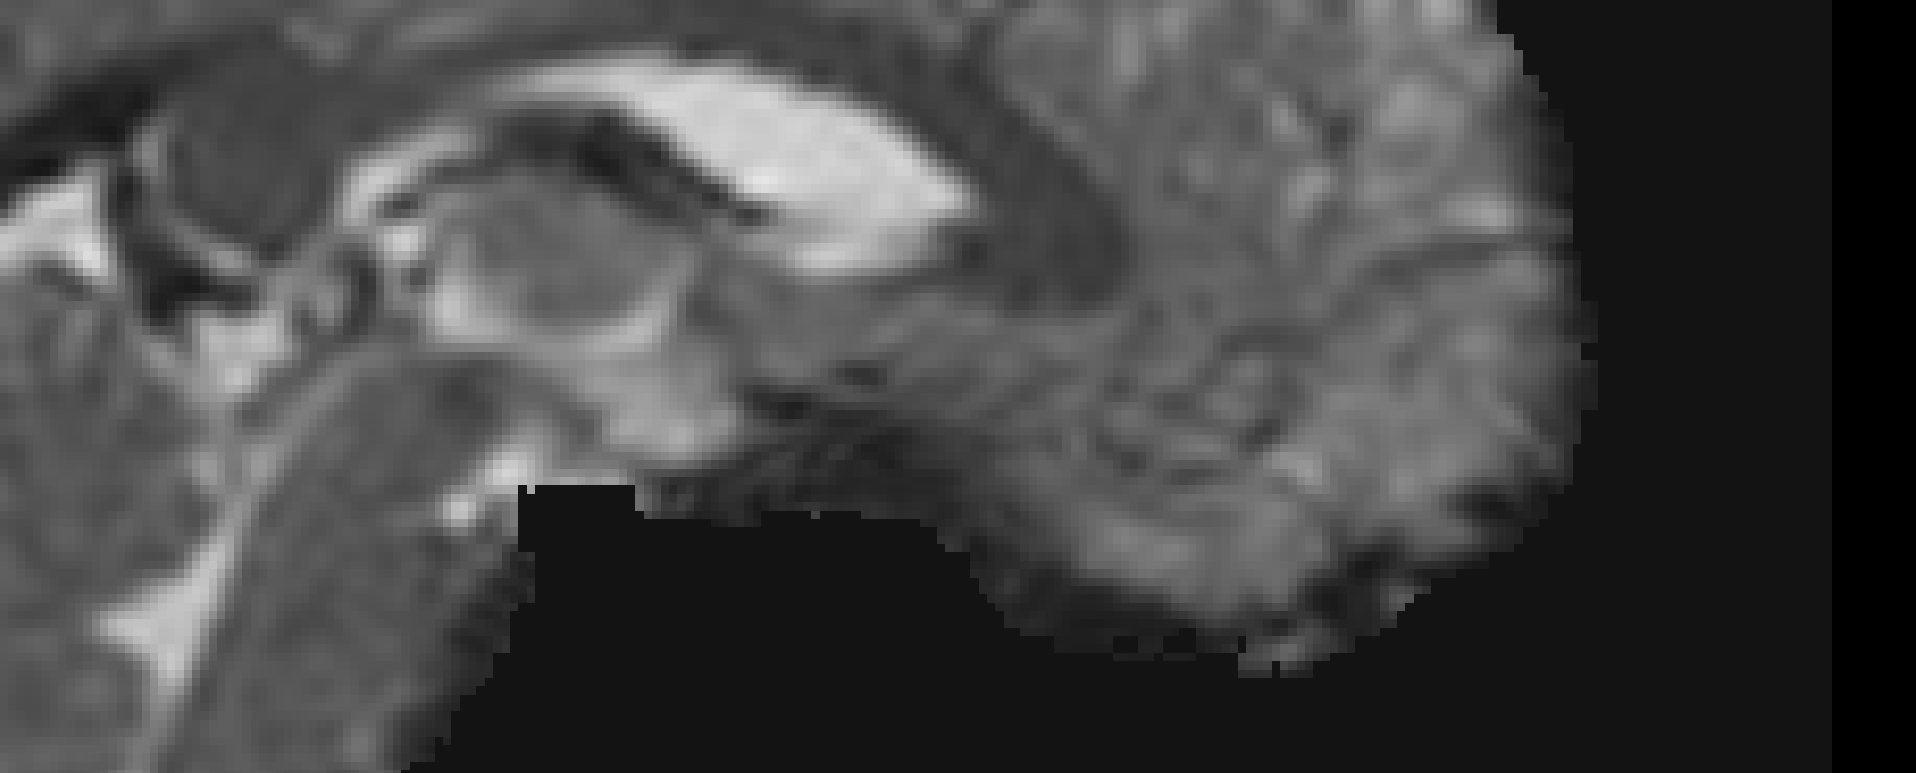
\includegraphics[width=\linewidth]{scout_zoom.png}%
\captionof{figure}[Zoomed in Scout\_gdc\_undistorted2T1w file]{Zoomed in version of part of checkerboard image marked with red square in Figure~\ref{fig:scout_gdc_file}}
\label{fig:scout_zoom}
\end{center}

\section{Effect of changing subject Vs. Changing condition}\label{sec:comparison}
In order to quantify the effect of operating system on the output image and to compare the difference with the anatomical differences between subjects, we made a comparison with two subjects processed in the same condition (101107 and 101006) vs. same subjects processed in two different conditions (CentOS6 and CentOS7). Subjects 101107 and 101006 processed using PreFreeSurfer on CentOS7 was compared against 101006, 101007 processed on CentOS6 and CentOS7 respectively. Table~\ref{tab:comparison_table} contains the mean, median and standard deviation across the said conditions.

\begin{center}
\begin{tabularx}{.98\textwidth}{|c|c|c|c|c|c|c|}
\hline
Item  & \makecell[l]{NRMSE\\(101006 \\ vs.\\101107)} & \makecell[l]{Dice Coeff.\\(101006\\ vs.\\101107)} & \makecell[l]{NRMSE\\101006\\CentOS\\(6Vs7)} & \makecell[l]{Dice Coeff.\\ 101006\\CentOS\\(6Vs7)} & \makecell[l]{NRMSE\\101107\\CentOS\\(6Vs7)} & \makecell[l]{Dice Coeff.\\ 101107\\CentOS\\(6Vs7)} \\ \hline
Average            & 0.092        & .265      & 0.0066     & 0.3014   & .0077   & .3001     \\ \hline
Median             & 0.078    & .0109       & 0.004          & 0.0217           & .0045     & .021  \\ \hline
\makecell[l]{Std.\\Dev} & 0.073     & 0.377           & 0.0092         & 0.3898   & .0100       & .385 \\ \hline
\end{tabularx}
\captionof{table}{Comparison: Anatomical differences vs. Effect of operating system}
\label{tab:comparison_table}
\end{center}

Comparing the metric values obtained from anatomical differences and effect of operating system differences, differences due to the effect of operating systems, quantified by NRMSE value on subject 101006, is 1/14\textsuperscript{th} (0.92/.0066) of the differences that are caused by the anatomical variations of the subjects (101006 vs. 101107). Similarly, the effect of operating system on subject 101107, is 1/12\textsuperscript{th} (0.092/.0077) of the differences that are caused by the anatomical variations of the subjects (101006 vs. 101107).

Analyzing the dice coefficient value of similarity in the same manner shows that the differences due to operating systems is so close to the differences due to anatomical variations (101006, dice coeff. ratio, .265/.30 = 0.88; 101107, dice coeff. ratio, .265/.30 = 0.88). The differences caused by anatomical variations in the subjects is 0.88 times the differences caused by operating system version updates. Thus, operating system updates are having a strong influence on the output images from the pipelines.
